
%%%%%%%%%%%%%%%%%%%%%%%%%%%%%%%%%%%%%%%%%%%%%%%%%%%%%%%%%%%%%%%%%%%%%%%%%%%%%
%% Descr:       Vorlage für Berichte der DHBW-Karlsruhe, Ein Kapitel
%% Author:      Prof. Dr. Jürgen Vollmer, vollmer@dhbw-karlsruhe.de
%% $Id: kapitel2.tex,v 1.5 2017/10/06 14:02:51 vollmer Exp $
%%  -*- coding: utf-8 -*-
%%%%%%%%%%%%%%%%%%%%%%%%%%%%%%%%%%%%%%%%%%%%%%%%%%%%%%%%%%%%%%%%%%%%%%%%%%%%%%%

\chapter{Umsetzung}
\label{chap:Umsetzung}
Dieses Kapitel greift die in der Konzeption (\ref{chap:Konzeption}) aufgeführten Planungen und Ideen auf und legt die Implementierung, bzw. 
Umsetzung detailliert dar. Darunter sind Lösungsansätze aufgezeigt und aufgetretene Probleme und deren Behebung dokumentiert. Allgemein zählt 
dazu die Umsetzung des Startmenüs und der beiden Kernfunktionen. Sowohl die Frontend- als auch die Backend-Aspekte werden in der Implementierung 
(\ref{chap:implementierung}) aufgezeigt. 

\section{Implementierung}
\label{chap:implementierung}
%Aufgrund der zuvor dargelegten Konzeption, ging es an die Umsetzung des Konzepts und an die Implementierung der Funktionen, die das System ausmachen. 
%Nachdem die Konzeption endgültig abgeschlossen war, ging es an die Umsetzung des Konzepts und an die Implementierung der Funktionen, die das System 
%ausmachen. 
%\\ 
Die Use Cases und deren Implementierung wurden nach logischer und chronologischer Reihenfolge entwickelt. % und dokumentiert. 
Diese festgelegte Reihenfolge ist auch der Abbildung (\ref{pic:anwendungsfall}) zu entnehmen. 
%Angefangen mit dem Startmenü, das dem Nutzer die Möglichkeit gibt, zwischen den Funktionen 
%zu wählen, folgte  die Implementierung der Scan-Phase, in der die realen Objekte virtualisiert und im Raum platziert werden. Zuletzt kam die Visualisierungs-Phase, 
%welche aufbauend auf die Scan-Phase funktioniert und die zuvor gescannten Objekte erneut virtuell im Raum einsetzt. 
%\\ 
%Beim ersten Gebrauch der Anwendung ist eine vorzeitige Nutzung der Visualisierungs-Phase ohne weiteres nicht möglich. Zuvor muss der Nutzer einen Scan durchführen, sodass 
%das System Daten generiert, Informationen liefert und diese zur Verfügung stellt. Dies hat zur Folge, dass die zweite Kernfunktion mit den zuvor erzeugten Informationen 
%durch die Scan-Phase operiert und ausgeführt werden kann. 
%\\ 
%\linebreak 
%Aufgeteilt wurden die Use Cases der Anwendung jeweils immer nach Frontend und Backend, demnach wird auch die Dokumentation in diesem Stil geschildert. 
\\ 
\linebreak
Gestartet wurde die eigentliche Implementierung mit der Aufgabe, die Entwicklungsumgebung zu wählen und einzurichten. 
Als \ac{IDE} wurde die speziell für Android-Applikationen entwickelte Software \textit{Android Studio} ausgesucht. Diese ist besonders für die Entwicklung von 
Android-Applikationen geeignet, d. h. es können nur Geräte anwenden, die das Android Betriebssystem nutzen. 
\\
Android Studio ist von Google LLC. und JetBrains entwickelt und basiert auf der IntelliJ IDEA Community Edition \acs{IDE}. Als 
Build-Management-Automatisierungs-Tool stellt Android Studio das Tool Gradle zur Verfügung, welches die zu bauenden Projekte durch die verwendeten 
Dependencies, Frameworks und Tools beschreibt. Um die notwendigen Libraries in einer Applikation verwenden zu können, werden in dieser Datei unter 
anderem die Bibliotheken und deren verwendete Version eingetragen. 
\\ 
\linebreak 
Bezogen auf das zu entwickelnden Unterstützungssystem wurden dort die Bibliotheken zur Nutzung der Android Architecture Components notiert, darunter 
Room und LiveData. 
Darüber hinaus wird an dieser Stelle auch die Version des ARCore Frameworks und des Sceneform \acs{SDK}s verwaltet, welche ebenso essentielle Bestandteile der 
Applikation sind.
\\ 
Nachdem alle Abhängigkeiten erfolgreich eingebunden waren, wurden zur übersichtlichen Gestaltung der Klassen, Objekte, ViewModel, Repositories und Activities 
eine Ordnerstruktur angelegt, die alle Klassen des gleichen Typs im Laufe der Entwicklung beinhalten sollten. Dadurch kann bei der Programmierung besser und 
übersichtlicher durch das Projekt navigiert werden. Es befinden sich alle Klassen ähnlicher Eigenschaften im selben Zielordner. 
\\ 
\linebreak
Damit im Laufe der Entwicklung die Applikation bestmöglich getestet werden konnte, war es notwendig, ein Testgerät zu verwenden. Mit dem verfügbaren 
Emulator\footnote{Ein System, das ein anderes in speziellen Teilbereichen nachbildet} von Android Studio konnte keine realitätsnahe Testung 
durchgeführt werden, deshalb wurde zum Testen der Anwendung ein Smartphone benutzt.
\\ 
\linebreak
Für die Designs der Benutzeroberflächen wurden Prinzipien der \ac{UX}, berücksichtigt. 
\\ 
Darunter folgende Punkte: 
\begin{itemize}
    \item Übersichtlichkeit (Digestibility): Auf einen Blick verstehen, worum es geht. Der User versteht intuitiv was zu tun ist.
    \item Klarheit (Clarity): Deutliche und verständliche Ausdrucksweise und klar herauszufindenden Nutzen der Funktion, bzw. Anwendung.
    \item Vertrauen (Trust): Gutes Design erlangt Vertrauen. Offenlegung der Aktionen und Hintergründe. 
    \item Begeisterung (Delight): Komplexe Sachverhalte einfach zu lösen. 
\end{itemize} 
\subsection{Startmenü}
Das Startmenü ist die zentrale Anlaufstelle des prototypischen Unterstützungssystems und bildet den Einstiegspunkt in die Interaktionen zwischen Anwender 
und dem Assistenzsystem. 
\subsubsection{Frontend}
Zuallererst werden bei initialer Instandsetzung bestimmte Genehmigungen eingeholt, um die Anwendung überhaupt starten zu können. Der Nutzer soll dem System 
die Zugriffserlaubnis auf die Kamera erteilen, da in der Hauptfunktion die Umgebung gescannt werden muss. 
Diese Abfrage erfolgt über ein kleines PopUp-Fenster, welches von Android fest vorgegeben ist. 
Mit dem Zulassen des Zugriffs auf die Kamera kann die geplante Fortführung der Applikation erfolgen. Somit wird sichergestellt, dass alle notwendigen Genehmigungen 
eingeholt werden.
\\ 
\linebreak
Da speziell das Assistenzsystem für das gegebene Betriebssystem entwickelt wurde, zählt dieses zu den nativen Applikationen. 
Darunter sind Anwendungen zu verstehen, die ausdrücklich für das Betriebssystem des Endgeräts konzipiert sind oder die zum Beispiel auf die vom Endgerät vorhandenen 
Komponenten zugreifen, wie in etwa auf die Bild-Mediathek, sämtliche Datei-Strukturen oder die Kamera-Komponente.
\\ 
\linebreak
Angenommen der Nutzer lässt den Zugriff auf die Kamera für das Assistenzsystem zu, dann startet die Applikation. % wie erwünscht. 
Darauffolgend ist das eigentliche Startmenü zu sehen. Diese Ansicht ist der nachfolgenden Abbildung (\ref{pic:startmenu}) zu entnehmen. Die 
Benutzeroberfläche weist ein sehr einfaches und schlicht gehaltenes Design auf. Dadurch wird dem Nutzer eine klare Struktur vorgelegt. 
Darauf ist das Firmen-Logo der cjt Systemsoftware AG zentriert zu sehen, außerdem zwei farblich voneinander getrennte Buttons zur Navigation innerhalb der Applikation. 
Die Buttons adressieren jeweils die nachfolgend zugehörige Funktion. Dies sind zum einen der lilafarbene Button, der zur Scan-Phase weiterleitet und zum anderen der 
gelbfarbene Button, der den Nutzer zur Visualisierungs-Phase navigiert. Damit wurde das Ziel, zur klaren Vorgabe der Entscheidungsvarianten der Startmenü-Oberfläche, 
erreicht.
\begin{figure}[hbt!]
    \centering
    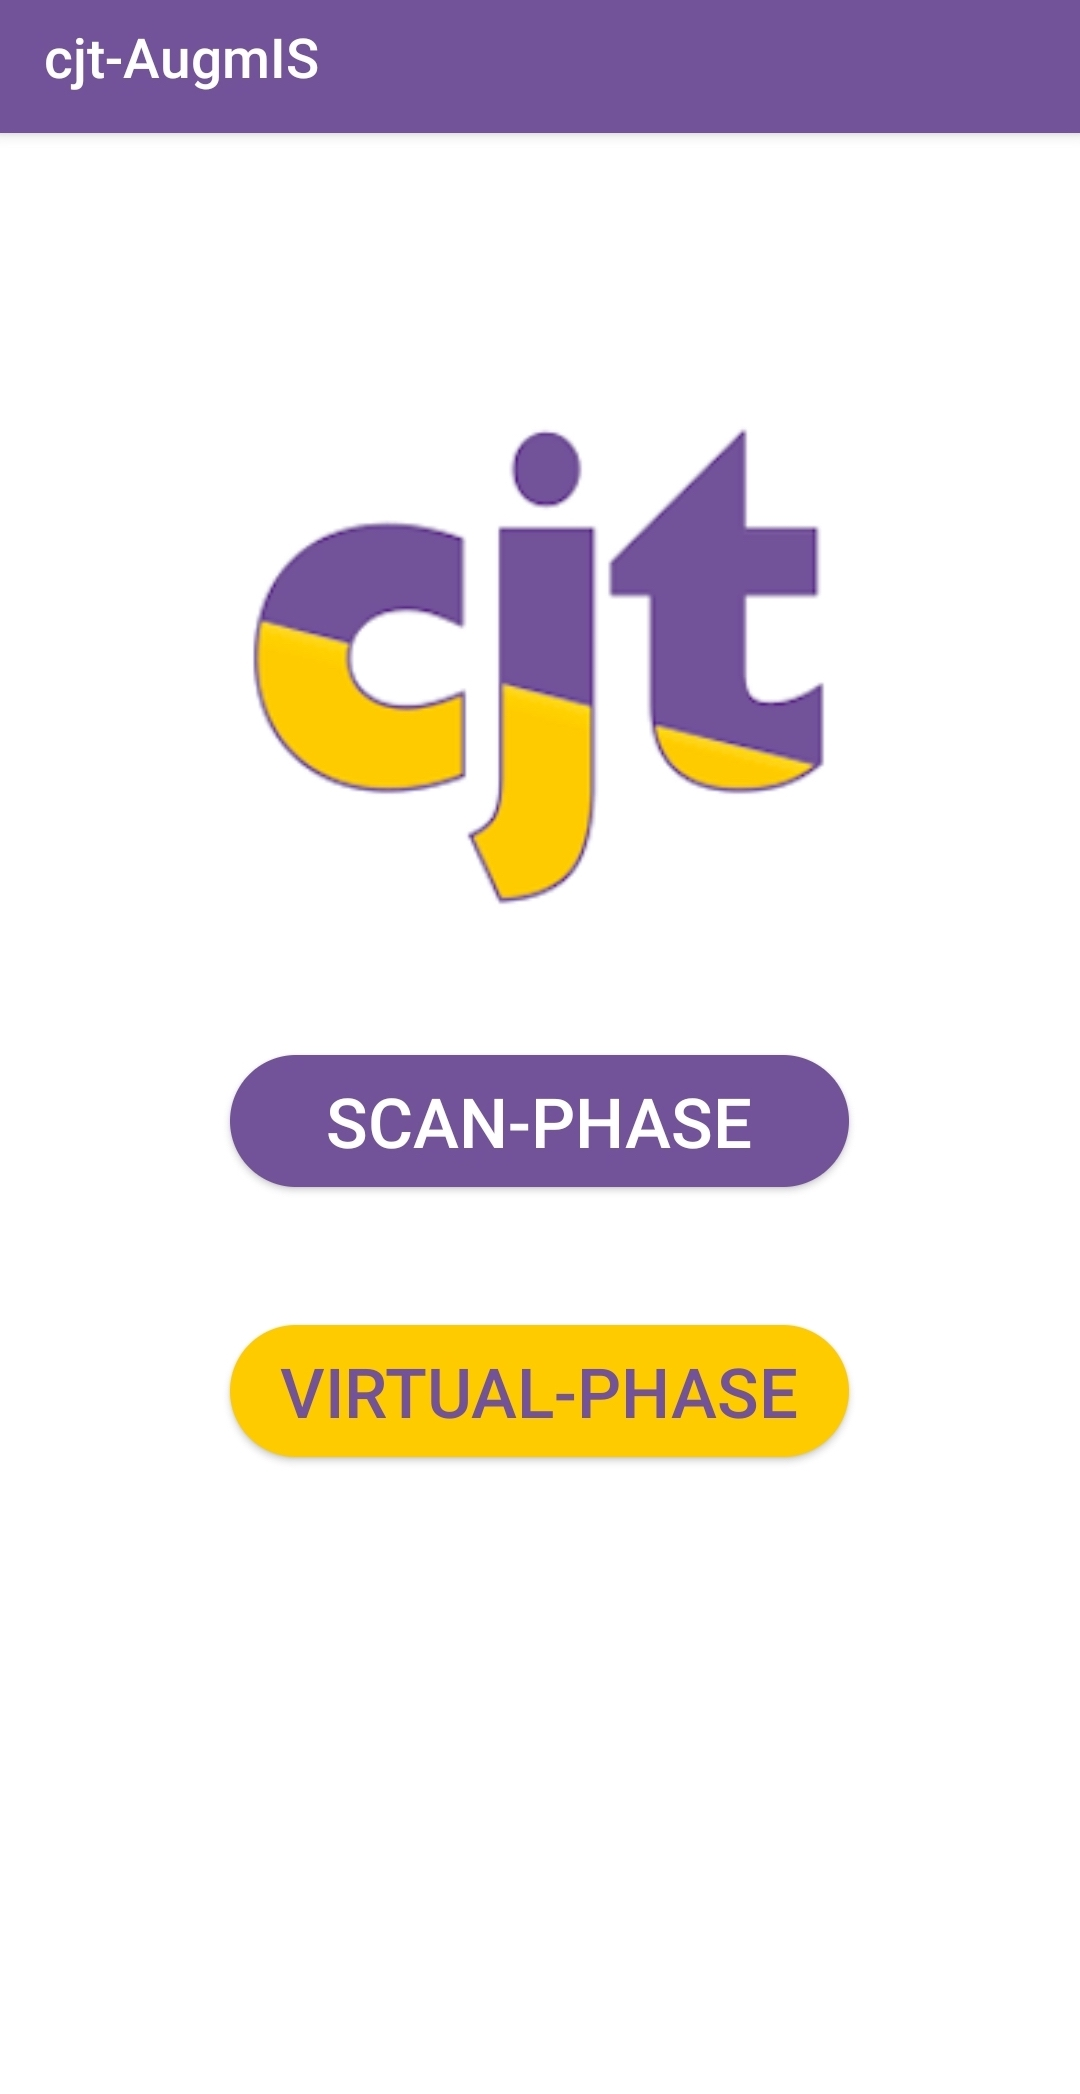
\includegraphics[width=7cm,height=7cm,keepaspectratio]{4Umsetzung/Bilder/startmenu.jpg}
    \caption{Startmenü der Applikation}
    \label{pic:startmenu}
\end{figure}
\\
Die Button-Interaktionen und die jeweils dahinterliegenden Funktionen sind durch den folgenden Programmablaufplan verdeutlicht. 
\begin{figure}[hbt!]
    \centering
    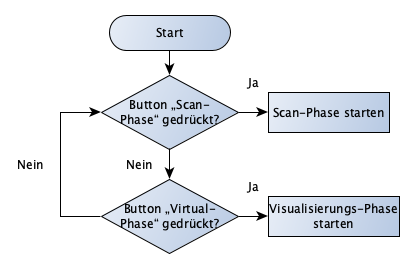
\includegraphics[width=8.5cm,height=8.5cm,keepaspectratio]{4Umsetzung/Bilder/startPAP.png}
    \caption{Programmablaufplan des Startmenüs}
    \label{pic:startmenu}
\end{figure}
\pagebreak
\subsubsection{Backend}
Durch die schlichte und einfach gehaltene Modellierung des Startmenüs zählt diese als Ansicht zum Einstieg in die Nutzung des Assistenzsystems, zur Abfrage der 
\textit{„Camera-Permission“} und zur weiteren Navigation innerhalb der Anwendung.
\\ 
Mit der \textit{„Permission-Request“} wird abgefragt, ob die Genehmigung zur Nutzung der Kamera in der \textit{„AndroidManifest.xml“}-Datei erteilt wurde, bzw. 
wird dadurch das PopUp-Fenster zur Nachfrage der Genehmigung geöffnet und die daraus resultierende Antwort in die Manifest-Datei eingetragen. 
\\ 
\linebreak
Die Manifest-Datei beinhaltet alle optionalen Metadaten, die für das Assistenzsystem benötigt werden. Dazu gehören die Google ARCore-Metadaten, sowie die 
grundlegenden Informationen über das Projekt, die das Android-System zum Installieren und Ausführen der Applikation fordert. Des Weiteren wird 
die Berechtigung zur Kameranutzung benötigt. Ebenso werden Angaben zu Activities, bzw. Benutzeroberflächen gemacht und Stammdaten, z.B. Titel, -bild und 
App-Icon, die das Projekt eindeutig spezifizieren, definiert.

\subsection{Scan-Phase} %Umgebungserkennung /
\label{chap:scan_implementation}
Die Idee hinter der Scan-Phase ist die Implementierung einer Methode, die es ermöglicht, das Umfeld über die Kamera wahrzunehmen und mit den gewonnenen 
Erkenntnissen über den Raum weiterarbeiten zu können. Basierend auf diesen Raumerkenntnissen werden die virtuellen Objekte platziert. 
\\ 
Zur Schaffung einer Grundlage, um die wichtigsten Funktionen zu implementieren, wurden zuallererst die Benutzeroberflächen erstellt. Diese dienen 
unter anderem dazu, den Fokus auf die Funktionsweise der eigentlichen Methode nicht zu verlieren. Demnach werden die entwickelten \acs{GUI}s nun aufgeführt 
und näher beschrieben, um Methoden des Backends im Anschluss besser nachvollziehen zu können.
\subsubsection{Frontend}
Zur Repräsentation des Kamerabildes wurde in die Benutzeroberfläche ein Fragment zur Vollbildkamera-Anischt eingebaut, damit eine \textit{\acs{AR}-Experience} 
stattfinden kann. Zur optimalen Erfassung einzelner Bilder oder Marker wurde das Fragment mit einem weißen Rahmen überlagert. Dieser erleichtert dem Nutzer die 
Handhabung des Smartphones und das Einfangen des Bildes, damit das Bild vollständig analysiert werden kann. 
%Das Assistenzsystem verfügt über eine Vollbildkamera-Ansicht, die mit einem weißen Rahmen überlagert ist. Damit können über die Kamera Bilder zentriert 
%eingefangen werden. Somit weiß der Nutzer, wie er das Smart-Device in Position bringen muss, damit er das zu scannende Bild über die Kamera optimal erfassen kann. 
\\ 
\linebreak
%Ursprünglich war die Applikation nicht mit diesem Layout der Abbildung (\ref{pic:image_tracking}) konzipiert, da während der Implementierung der Scan-Phase eine 
%schwerwiegende Änderung vorgenommen werden musste. Diese wird in dem Abschnitt der Scan-Phasen-Backend-Entwicklung zu gegebenem Zeitpunkt 
%aufgegriffen und genauestens dargelegt. 
Da ursprünglich die Applikation nicht mit dem weißen Rahmen konzipiert war, musste die Anwendung um dieses Layout (Abbildung \ref{pic:image_tracking}) 
ergänzt werden. 
\begin{figure}[hbt!]
    \centering
    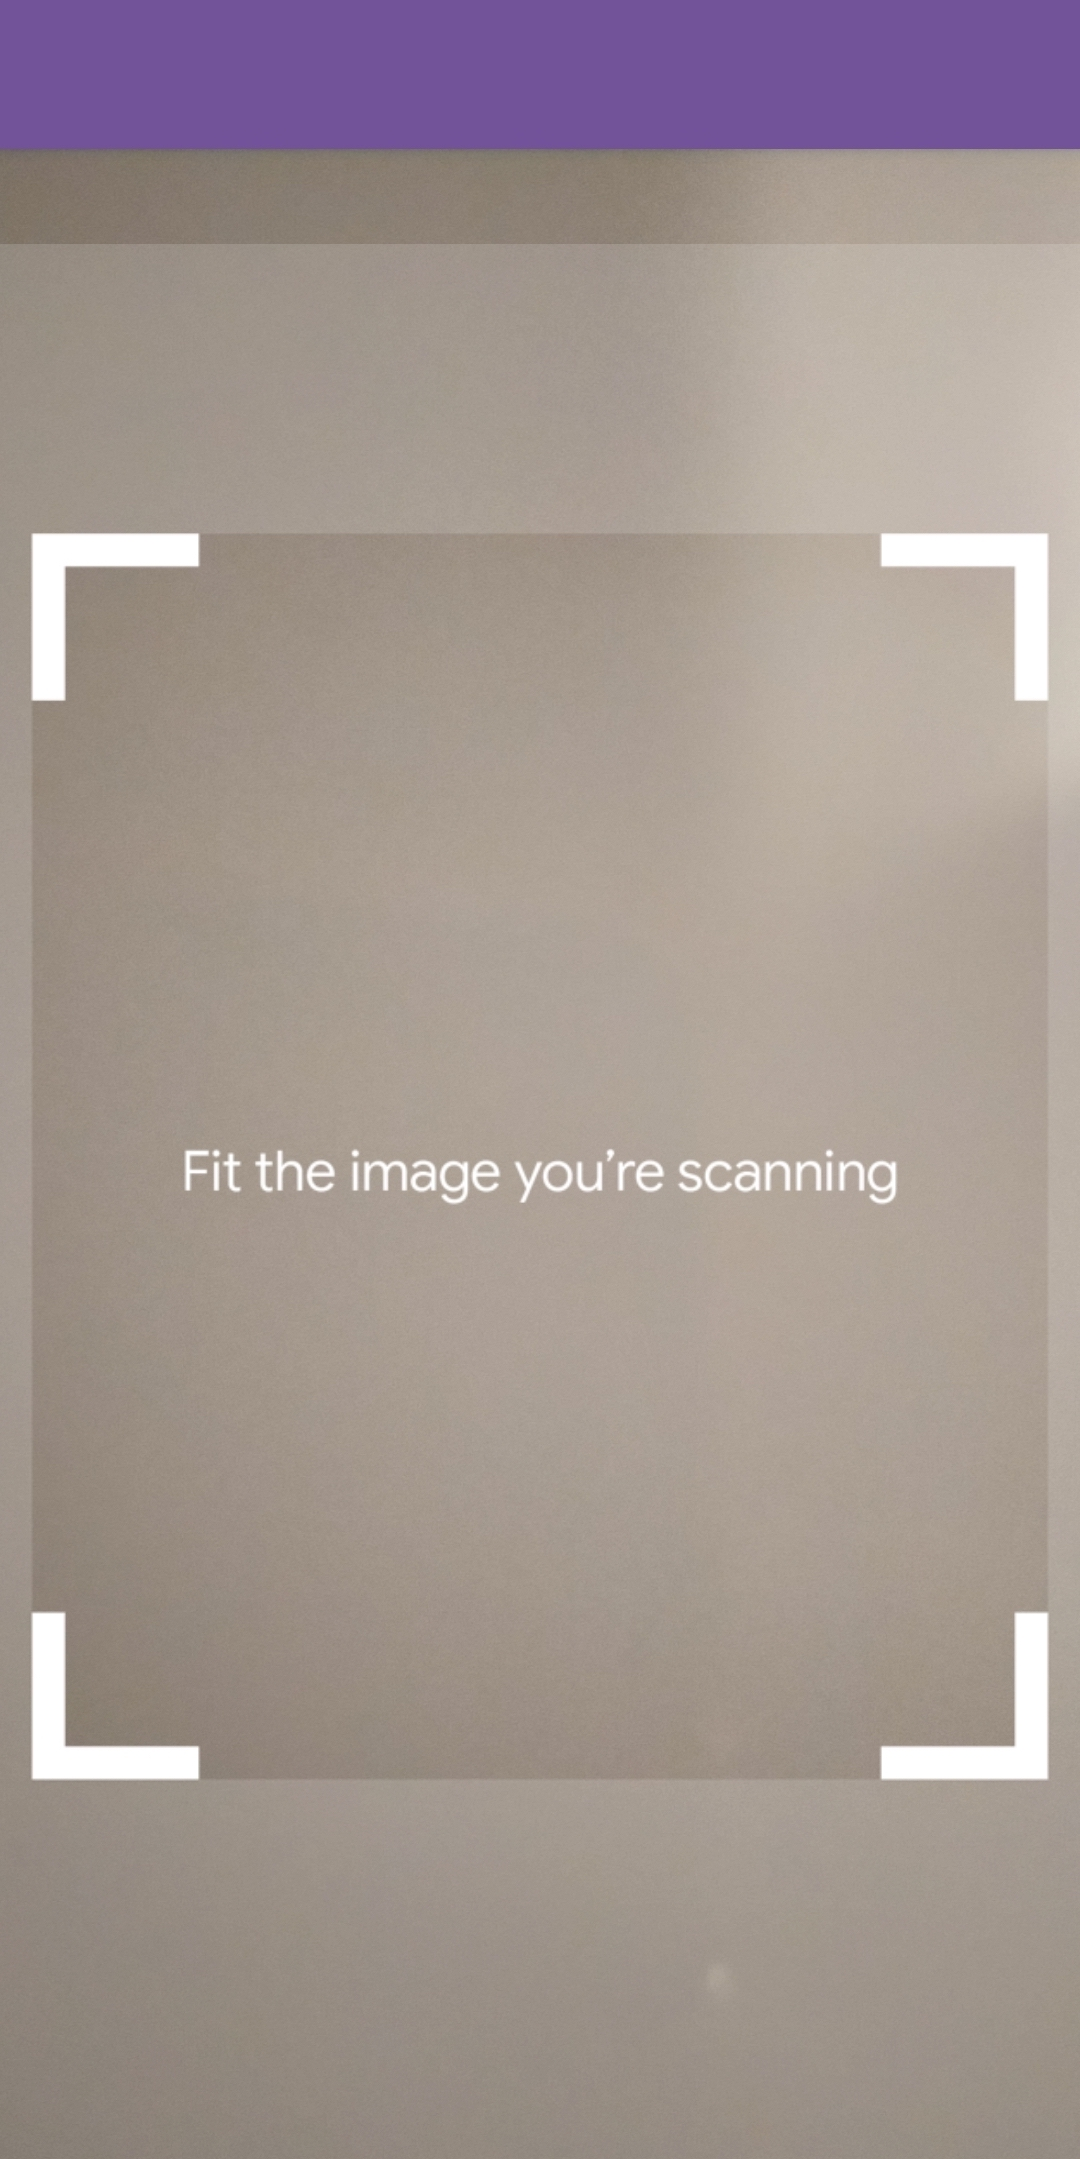
\includegraphics[width=7cm,height=7cm,keepaspectratio]{4Umsetzung/Bilder/image_tracking.jpg}
    \caption{Markererkennung der Applikation zum Start der Scan-Phase}
    \label{pic:image_tracking}
\end{figure}
\pagebreak 
\\ %%%%%%%%%%%%%%%%%%%%%%%%%%%%%%%%%%%%%%%%%%%%%%%%%%%%%%%%%%%%%%%%%%%%%%
Des Weiteren beinhaltet das Assistenzsystem die eigentliche Scan-Phasen \acs{UI}, mit der die Umgebung aufgenommen wird und anhand dieser Daten 
der Nutzer die Objekte an von ihm definierte Stellen platzieren kann. Die Benutzeroberfläche hat ein schlichtes und überschaubares Layout, damit der Nutzer den 
Überblick nicht verliert und sich auf die eigentliche Funktion konzentriert. 
\\ 
Hauptsächlich beinhaltet die \acs{GUI} ein Fragment, welches das Kamerabild in Echtzeit wiedergibt. Am oberen Ende des Bildschirms, bzw. der Abbildung 
(\ref{pic:scan}) wurde eine lilafarbene Fläche zur optischen Abgrenzung integriert. Sie soll gleichzeitig zur Anzeige von Informationen dienen. Dadurch ist eine 
Möglichkeit geschaffen dem Nutzer Mitteilungen oder Updates der Anwendung einzublenden. 
\\ 
Am unteren Ende des Bildes befindet sich eine \textit{„Android-Gallery“}, die alle zu platzierenden Objekte beinhaltet. Der Gedanke dabei war, eine einfache 
Bedienung der Buttons zu gewährleisten. In der zugrundeliegenden Abbildung sind es zwei Platzhalter-Objekte, die bei Berührung des Bildes erstellt werden. 
Prinzipiell ist diese Gallery um beliebig viele Objekte erweiterbar. Diese Erweiterung erfolgt allerdings nicht dynamisch, sondern muss über manuelles 
Einfügen im Code stattfinden. 
\\ 
\linebreak
Um weiterhin auf der Seite navigieren zu können, gibt es im rechten unteren Eck einen weiteren Button, welcher ebenso der Abbildung (\ref{pic:scan}) 
zu entnehmen ist. Diese Schaltfläche leitet den Nutzer weiter, bzw. wieder zurück zum Startmenü und beendet die Scan-Phase. 
\\ 
\linebreak
Damit der Nutzer über die in der Datenbank gespeicherten Informationen Modifizierungsmöglichkeiten besitzt, gibt es im linken oberen Eck der \acs{UI} eine 
zusätzliche Schaltfläche mit einem roten Kreuz versehen. Der Nutzer kann somit alle vorhandenen in der Datenbank persistierten Informationen löschen 
und den Scan-Vorgang von der ursprünglichen Ausgangsposition erneut beginnen. %%%%%%%%%%%%%%%%%%%%%%%%%%%%%%%%%%%%%%%%%%%%%%%%%%%%%%%%%%%%%%%%%%%%%%%%%%%%%%%
\begin{figure}[hbt!]
    \centering
    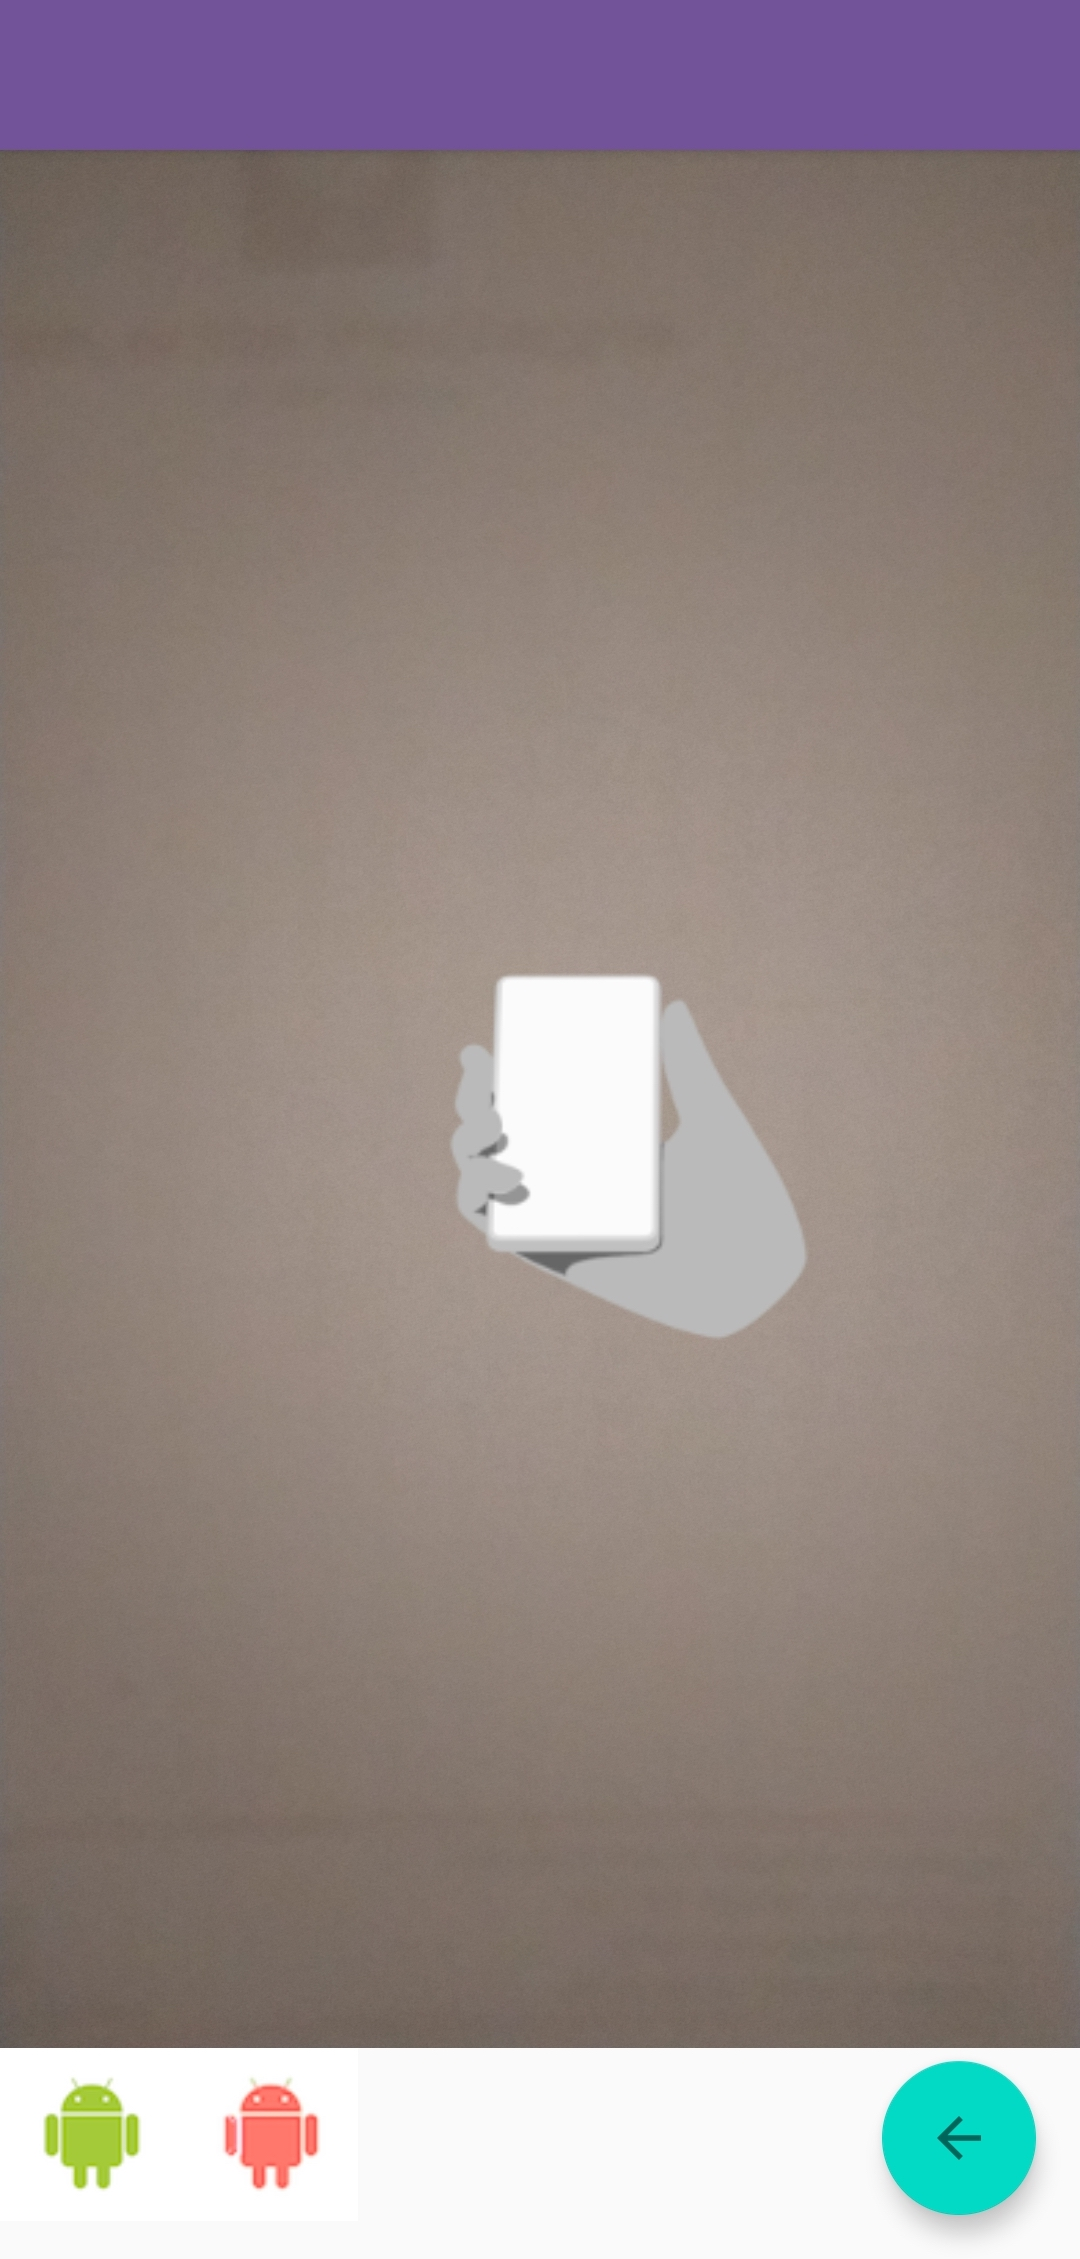
\includegraphics[width=7cm,height=7cm,keepaspectratio]{4Umsetzung/Bilder/scan-phase.jpg}
    \caption{Scan-Phase der Applikation}
    \label{pic:scan}
\end{figure}
\pagebreak
\\
Will der Anwender ein Objekt erstellen und danach zusätzliche Informationen hinzufügen, muss er den entsprechenden Button mit dem Objekt drücken, der 
dieses repräsentiert. Daraufhin wird eine weitere \acs{UI} sichtbar, in der die dazugehörigen Informationen vom Nutzer eingetragen und anschließend 
%die der Nutzer die dazugehörigen Informationen einträgt und die anschließend 
in die Datenbank aufgenommen werden. Die zusätzliche Eingabe von Informationen wurde so umgesetzt, dass bei Betätigen des Buttons die Oberfläche zur 
Texteingabe erscheint. Die \acs{UI} wurde mit einem \textit{„save“}-Button versehen, damit die Informationseingaben in die Datenbank stattfindet. % und gespeichert wird.
%abdecken. 
\\ 
Im Hintergrund werden ebenso die Daten der Position und Drehung des 
Objekts bereitgestellt, die mit den Informationen des Objekts persistiert werden.
\\ 
\linebreak
Anhand des folgenden Plans wird der Ablauf der Scan-Phase veranschaulicht.
\begin{figure}[hbt!]
    \centering
    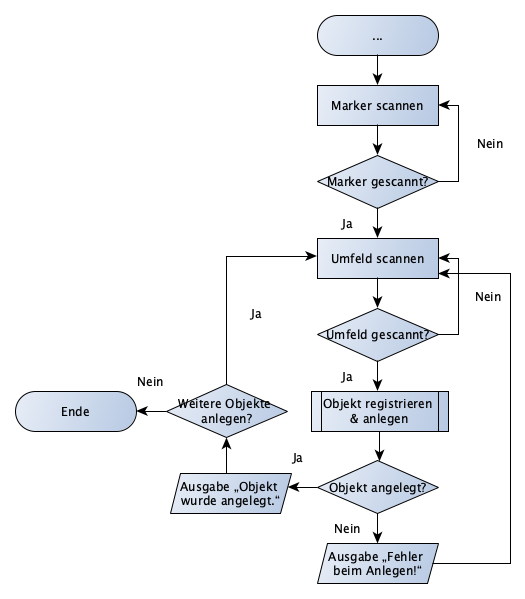
\includegraphics[width=15cm,height=15cm,keepaspectratio]{4Umsetzung/Bilder/scanPAP.png}
    \caption{Programmablaufplan der Scan-Phase}
    \label{pic:startmenu}
\end{figure}